
\begin{figure*}[!ht]
    \centering
    \vspace{-3mm}
	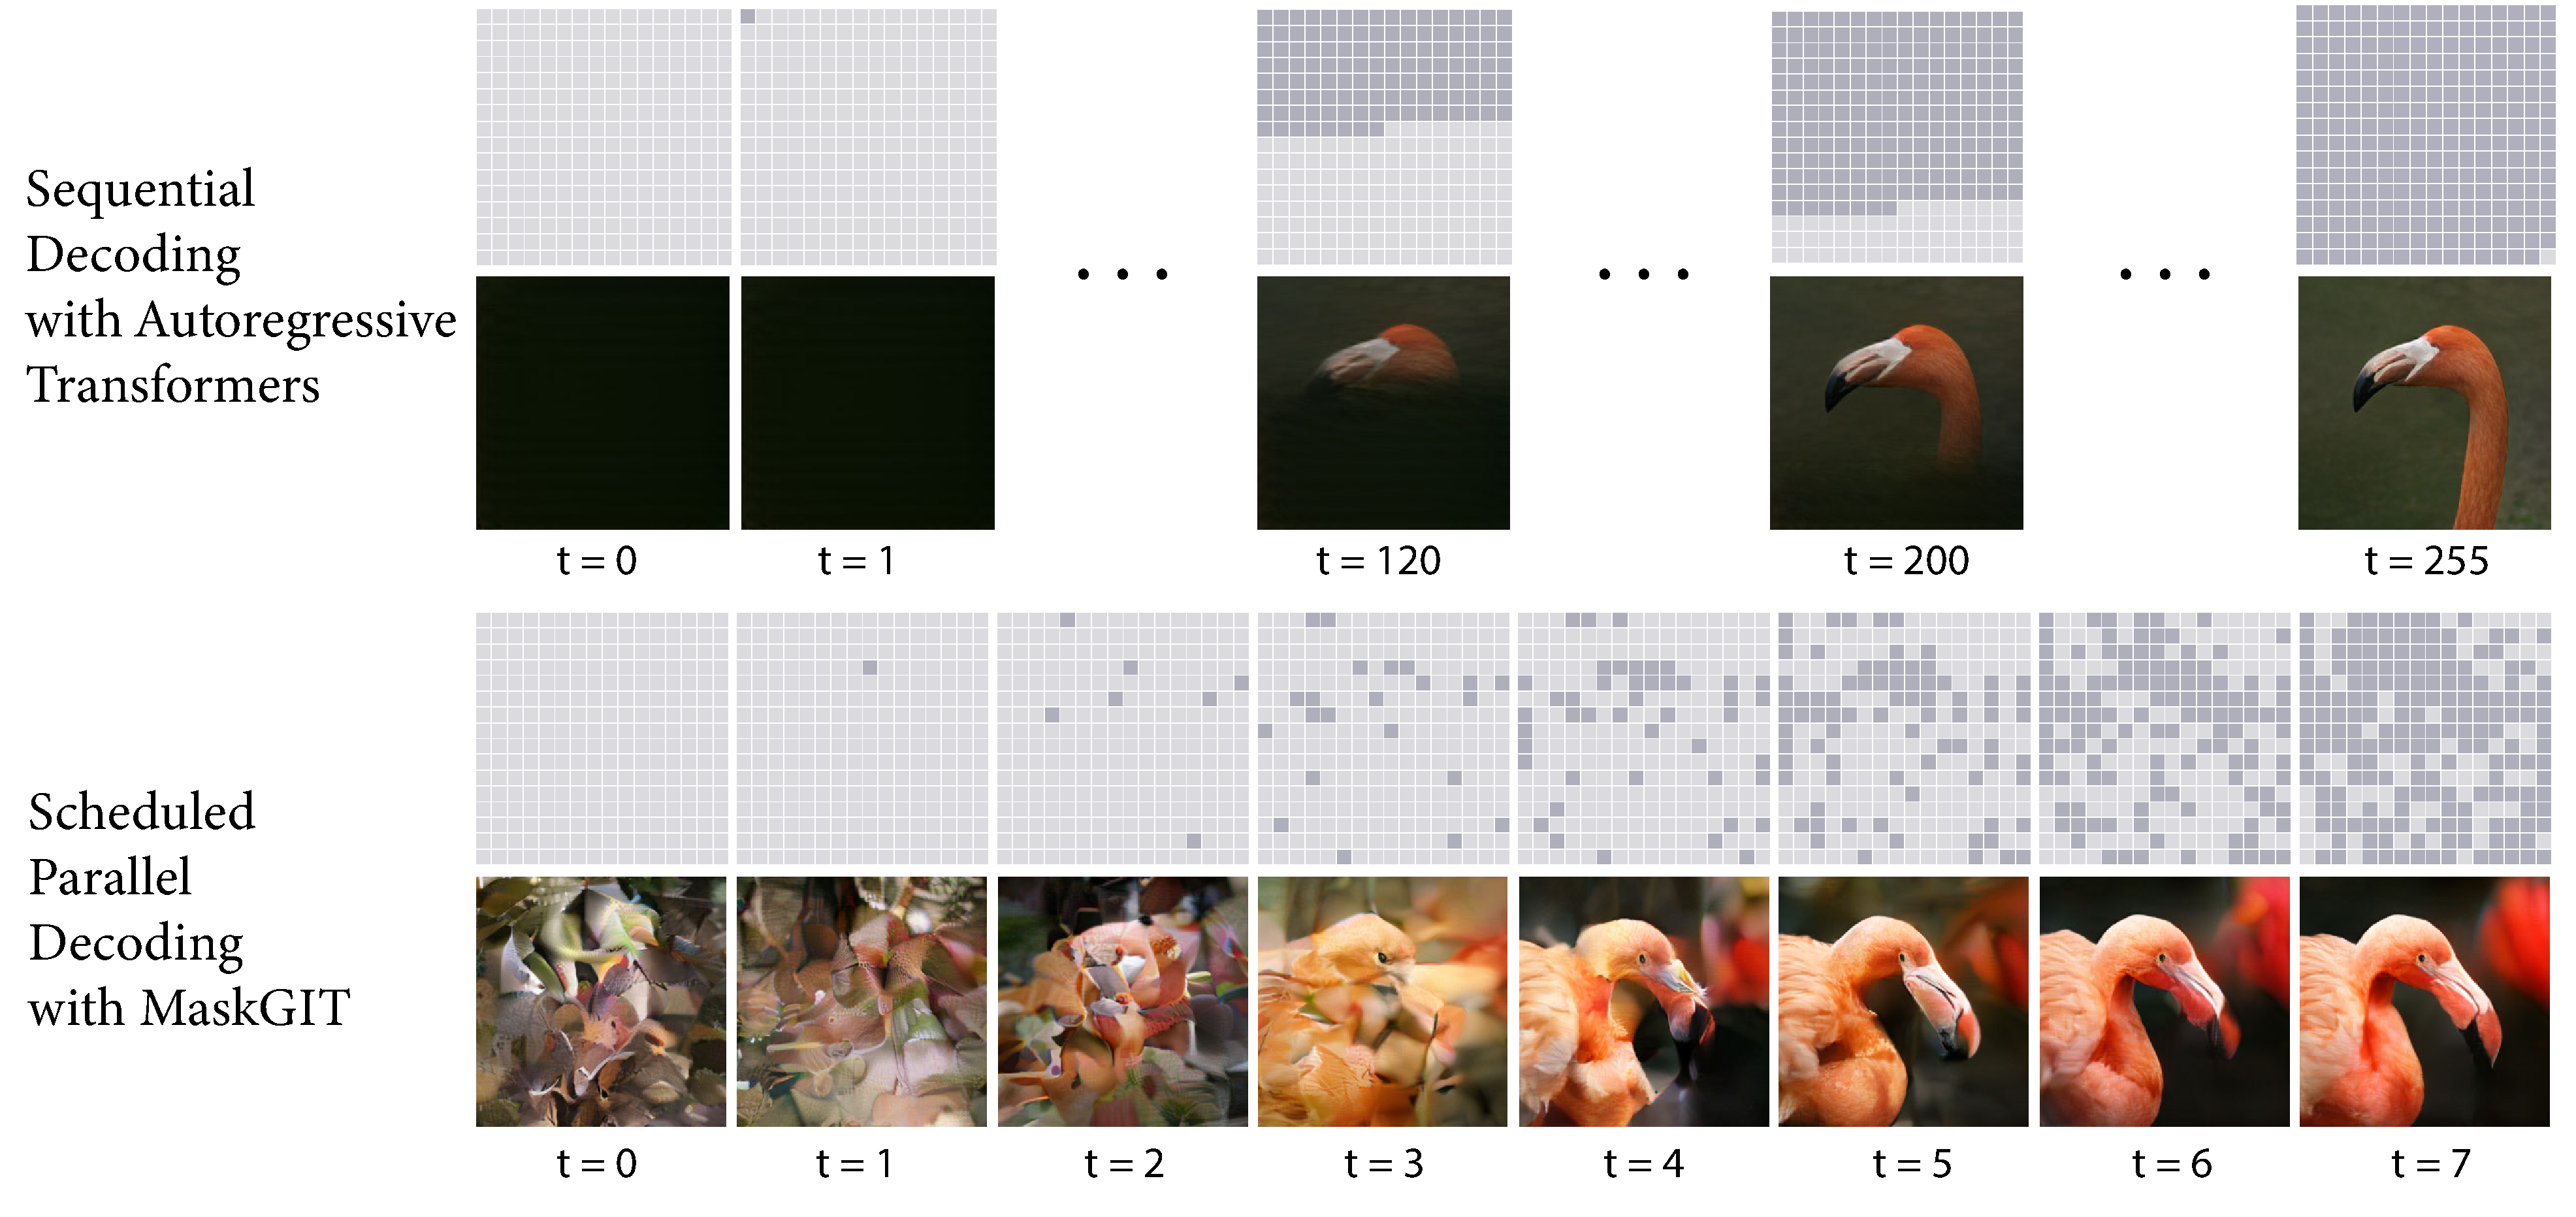
\includegraphics[width=.9\textwidth]{figures/iterative_decoding.pdf}
    \vspace{-3mm}
    \caption{\textbf{Comparison between sequential decoding and \model's scheduled parallel decoding.} Rows 1 and 3 are the input latent masks at each iteration, and rows 2 and 4 are samples generated by each model at that iteration. Our decoding starts with all unknown codes (marked in lighter gray), and gradually fills up the latent representation with more and more scattered predictions in parallel (marked in darker gray), where the number of predicted tokens increases sharply over iterations. \model finishes its decoding in 8 iterations compared to the 256 rounds the sequential method takes.}
    \label{fig:decoding}
\vspace{-3mm}
\end{figure*}